
\textbf{Definition Stetigkeit:}\\
$\forall \epsilon > 0 :\exists \delta > 0 : |x-a|<\delta : |f(x)-f(a)|<\epsilon$\\
$\forall \epsilon > 0 :\exists \delta > 0 : f(U_{\delta}(a) \subseteq U_{\epsilon}(f(a)))$\\
$\forall \epsilon > 0\  \exists \delta >0 : \text{sodass aus } |x-a|<\delta \text{ stets } |f(x)-f(a)|<\epsilon \text{ folgt}$\\

\textbf{Definition Unstetigkeit:} $\exists \epsilon > 0 \forall\  \delta > 0 :\exists x \in D : |x-x_0|< \delta \wedge |f(x)-f(x_0)|>\epsilon$

\subsection{links-rechtsseitiger Grenzwetz:}

$\lim\limits_{x\to x_0^-}f(x) = \lim\limits_{x\to x_0^+} f(x)$

$x_0$ wird von rechts und links angenähert. Sind beide Grenzwerte gleich ist die Funktion stetig.


\subsection{$\epsilon - \delta$ Kriterium}

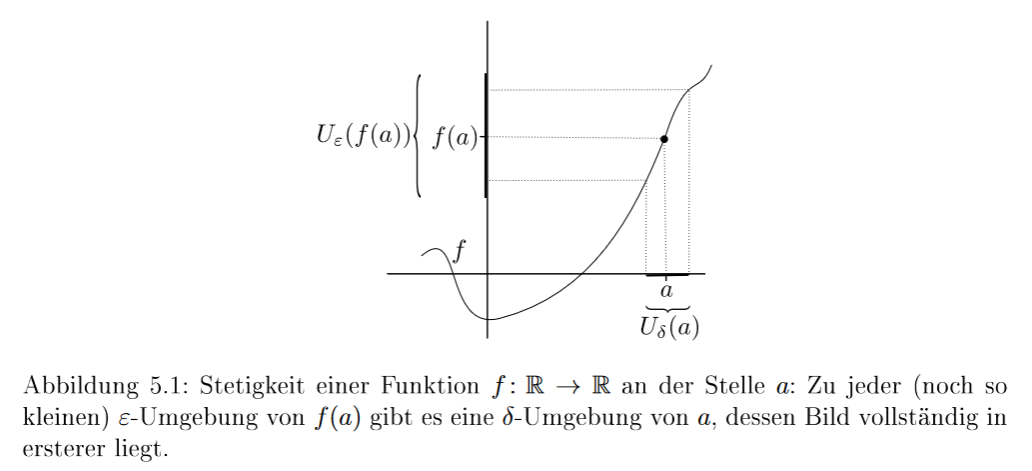
\includegraphics[width= \textwidth]{./pictures/Stetigkeit.png}
$\epsilon$ quer darf nach oben abgeschätz werden.
Zuerst delta ausrechnen
dann Beweis nochmal schön hinschrieben.\\

$|x-a|<\delta$\\
$|f(x)-f(a)|< \epsilon|$\\

$\epsilon$ darf gewählt werden

Nicht Stetigkeit beweisen:\\
>links und rechtsseitiger Grenzwert\\
>epsilon delta Kriterium

-->

$\exists \epsilon > 0 :\forall \delta >0 \exists x |x-x_0| < \delta \vee |f(x)-f(x_0) > \epsilon|$

